\documentclass[10pt]{beamer}
%\documentclass[handout]{beamer}

%\usepackage[en]{babel}

% TODO: debug warning messages
\usepackage{listings}           % used for TODO
\usepackage{color, colortbl}    % used for TODO
\usepackage{beamerthemeshadow}  % used for TODO
\usepackage{amsmath}            % used for mathematics
%\usepackage{arevmath}           % arevmath nice mathematical font, bold, simple
\usepackage{commath}            % used for TODO
\usepackage{float}              % used for TODO
\usepackage{multimedia}         % used for movie files, alternative: \usepackage{movie15}
\usepackage{hyperref}           % used for links to external players/browsers
%\usepackage{lmodern}
%\usepackage{helvet}
%\usepackage[T1]{fontenc}
%\renewcommand{\sfdefault}{cmss} % cmss: sans-serif, modern
% Futura and Gill Sans (Keynote's default font) Calibri (PowerPoint's
% default in their latest version) is nice. Gotham is a very popular
% font
%\renewcommand{\sfdefault}{helvetic}
%\renewcommand{\sfdefault}{gillsans} % gill sans (keynote default)
% \renewcommand{\sfdefault}{calibri} % PowerPoint default
%\renewcommand{\sfdefault}{futura}
%\renewcommand{\sfdefault}{gotham}

\beamersetuncovermixins{\opaqueness<1>{25}}{\opaqueness<2->{15}}
%\bibliographystyle{apalike}
%\bibliographystyle{plain}



\usetheme{Rochester}
\usecolortheme{beaver}
%\setbeamercolor{block itemize}{fg=red}
\setbeamercolor*{item}{fg=darkred} % all frames will have red bullets
\setbeamercolor*{title}{bg=darkred}

\beamertemplatenavigationsymbolsempty

%\pgfdeclareimage[height=0.5cm]{logo}{eth-logo}
%\logo{\pgfuseimage{logo}}

\setbeamertemplate{footline}
{%
  \leavevmode%
  \hbox{\begin{beamercolorbox}[wd=1\paperwidth,ht=1.ex,dp=0.5ex,%
                leftskip=.3cm,rightskip=.3cm]{white}%
    \usebeamerfont{author in head/foot}\insertshortinstitute\hfill\insertsection
  \end{beamercolorbox}}%
  \vskip0pt%
  \hbox{\begin{beamercolorbox}[wd=1\paperwidth,ht=1.5ex,dp=1.125ex,%
                leftskip=.3cm,rightskip=.3cm]{white}%
    \usebeamerfont{author in head/foot}\insertshortauthor\hfill\insertshorttitle, \insertshortdate\quad$|$ \insertpagenumber/\insertpresentationendpage
  \end{beamercolorbox}}%
  \vskip0pt%
}

\setbeamertemplate{headline}[text line]
{%
}

\setbeamertemplate{frametitle}
{
  \leavevmode
  \vskip0.45em
  \hbox{%
  \begin{beamercolorbox}[wd=0.93\paperwidth,ht=0.5ex,dp=0.ex]{frametitle}%
    \raggedright\hspace*{1em}\bfseries\insertframetitle
  \end{beamercolorbox}
  \vskip-0.4em
  }%
}

\usebackgroundtemplate{

\includegraphics[width=\paperwidth]{src/ETH_bg_caption.jpg}
}

\setbeamercolor*{title page}{fg=white}
\setbeamercolor{frametitle}{fg=black,bg=white}
\setbeamercolor{math text}{fg=darkred}

\makeatletter
\defbeamertemplate*{title page}{mytitlepage}[1][]
{
  \vbox{}
%  \vfill
  \vskip13em%
  \begin{centering}
    \begin{beamercolorbox}[sep=8pt,center,#1]{}
      \usebeamerfont{title}\bfseries\inserttitle\par%
      \ifx\insertsubtitle\@empty%
      \else%
        \vskip0.25em%
        {\usebeamerfont{subtitle}\usebeamercolor[fg]{subtitle}\insertsubtitle\par}%
      \fi%     
    \end{beamercolorbox}%
    \vskip1em\par
    \begin{beamercolorbox}[sep=8pt,center,#1]{author}
      \usebeamerfont{author}\bfseries\insertauthor
    \end{beamercolorbox}
    \begin{beamercolorbox}[sep=8pt,center,#1]{institute}
      \usebeamerfont{institute}\insertinstitute
    \end{beamercolorbox}
    \begin{beamercolorbox}[sep=8pt,center,#1]{date}
      \usebeamerfont{date}\insertdate
    \end{beamercolorbox}\vskip0.5em
    {\usebeamercolor[fg]{titlegraphic}\inserttitlegraphic\par}
  \end{centering}
  \vfill
}
\makeatother



% Some definitions for the priors:
\def\gprior{{\tt gprior}}
\def\cprior{{\tt cprior}}
\def\bprior{{\tt bprior}}
\def\lbprior{{\tt lbprior}}

%Some definitions for rhodm etc:
\def\vztwo{\overline{v_z^2}}
\def\vztwoi{\overline{v_{z,i}^2}}
\def\rhodisc{\rho_\mathrm{disc}(z)}
\def\rhodmext{\rho_\mathrm{dm,ext}}
\def\rhodm{\rho_\mathrm{dm}}
\def\rhoeff{\rho_\mathrm{dm}^\mathrm{eff}}
\def\nuobs{\nu_\mathrm{obs}(z)}

\def\ltsima{$\; \buildrel < \over \sim \;$}
\def\simlt{\lower.5ex\hbox{\ltsima}}
\def\gtsima{$\; \buildrel > \over \sim \;$}
\def\simgt{\lower.5ex\hbox{\gtsima}}
\def\siglos{\sigma_{\text{LOS}}}
\def\siglosi{\sigma_{\text{LOS},i}}
\def\kaplos{\kappa_{\text{LOS}}}

% units for inside math environments
\def\keV{\mathrm{keV}}
\def\MeV{\mathrm{MeV}}
\def\GeV{\mathrm{GeV}}
\def\Msun{M_{\odot}}
\def\pc{\mathrm{pc}}
\def\kpc{\mathrm{kpc}}
\def\Mpc{\mathrm{Mpc}}
\def\K{\mathrm{K}}


\title[Generations in Bounded Confidence]{Generations in Bounded
  Confidence Models}
\author{Pascal S.P. Steger}
\institute{ETH Zurich}
\date{\today}


\begin{document}

\begingroup
\setbeamertemplate{background canvas}{
  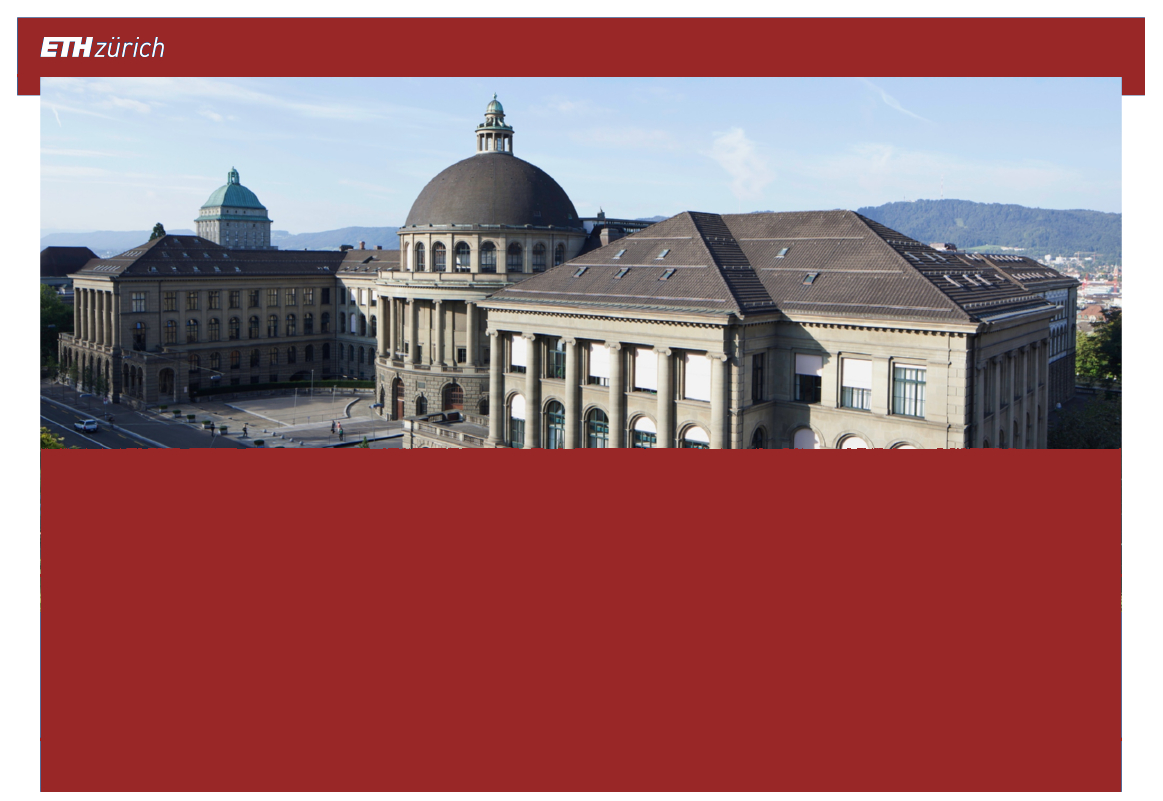
\includegraphics[width=\paperwidth]{src/ETH_bg.jpg}
}
%\titlegraphic{\usebackgroundtemplate{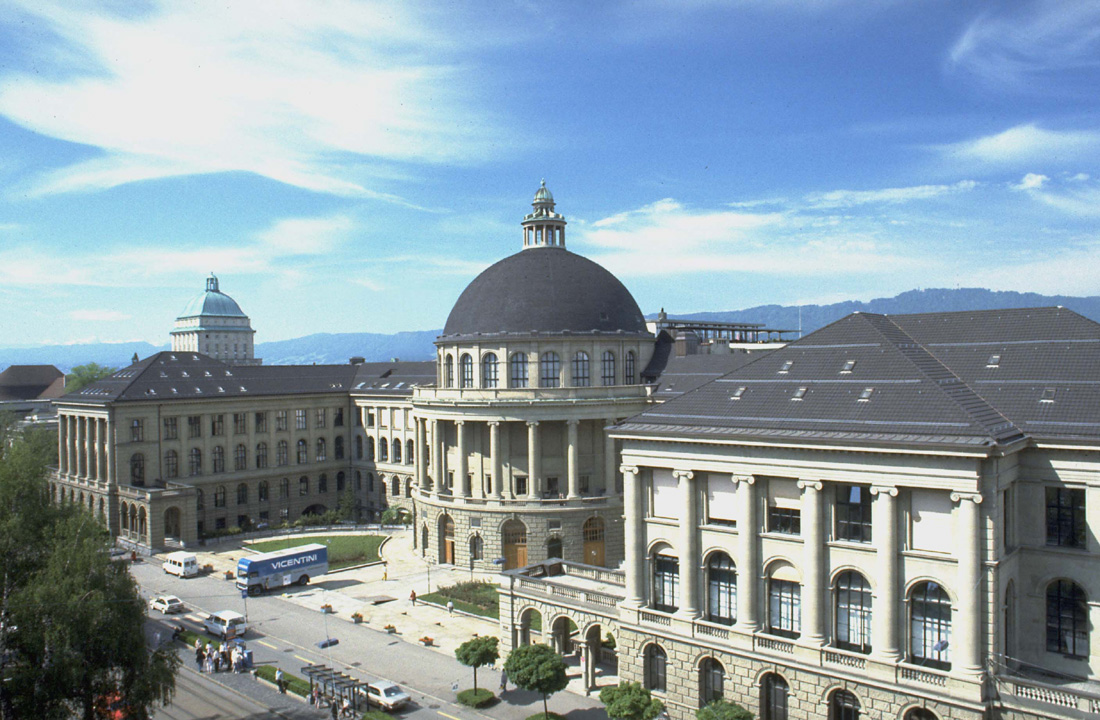
\includegraphics[width=0.8\textwidth]{src/ETH.jpg}}}
\begin{frame}
\maketitle
\end{frame}
%\begin{frame}
%    \titlepage
%\end{frame}
\endgroup


\section{Motivation} \label{sec:motivation}

\subsection{Change of Opinions}
\begin{frame}\frametitle{Change of Opinions}
    \begin{center}
        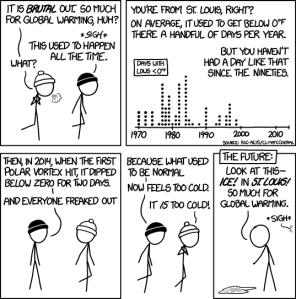
\includegraphics[height=0.8\textheight]{src/opiniondynamics}
    \end{center}
    
%    \talk{ Welcome. If you were president, and would like to change
%      the opinion of people quickly, you need to make sure that they
%      either do not talk to each other or that they die young. I will
%      explain why.
%    }

\end{frame}


\section{Model}
\begin{frame}\frametitle{Model}
    % left: equations

    % right: picture
    \begin{center}
        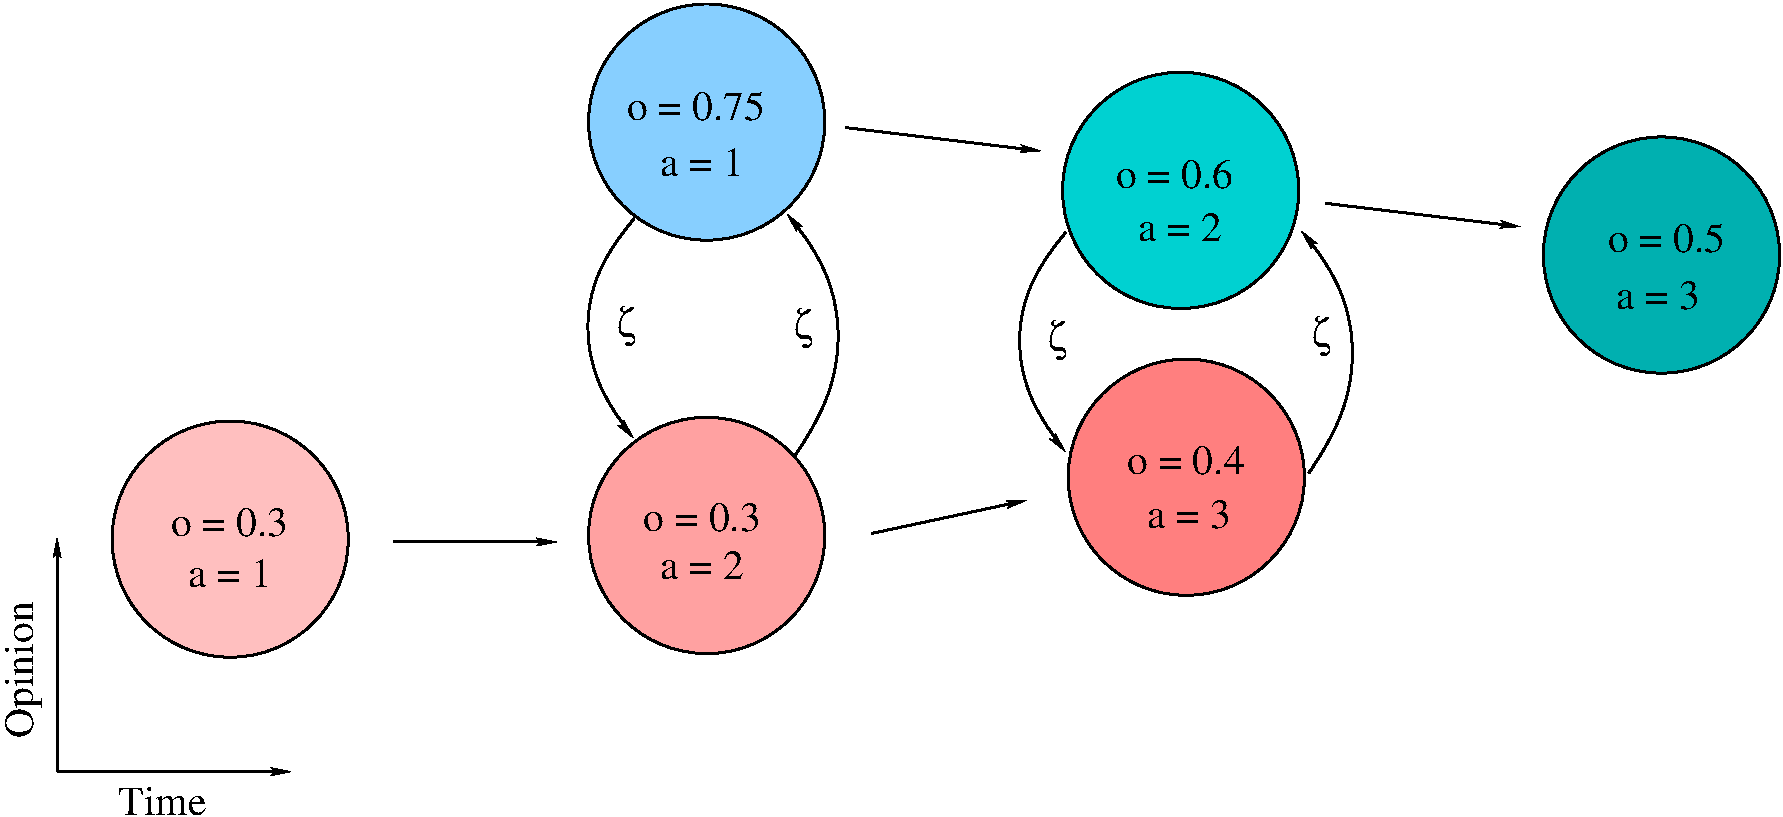
\includegraphics[width=0.9\textwidth]{src/internals.pdf}
    \end{center}
    
%    \talk{ I include one additional parameter, the age of an agent}

\end{frame}


\begin{frame}\frametitle{Evolution}
    \begin{center}
        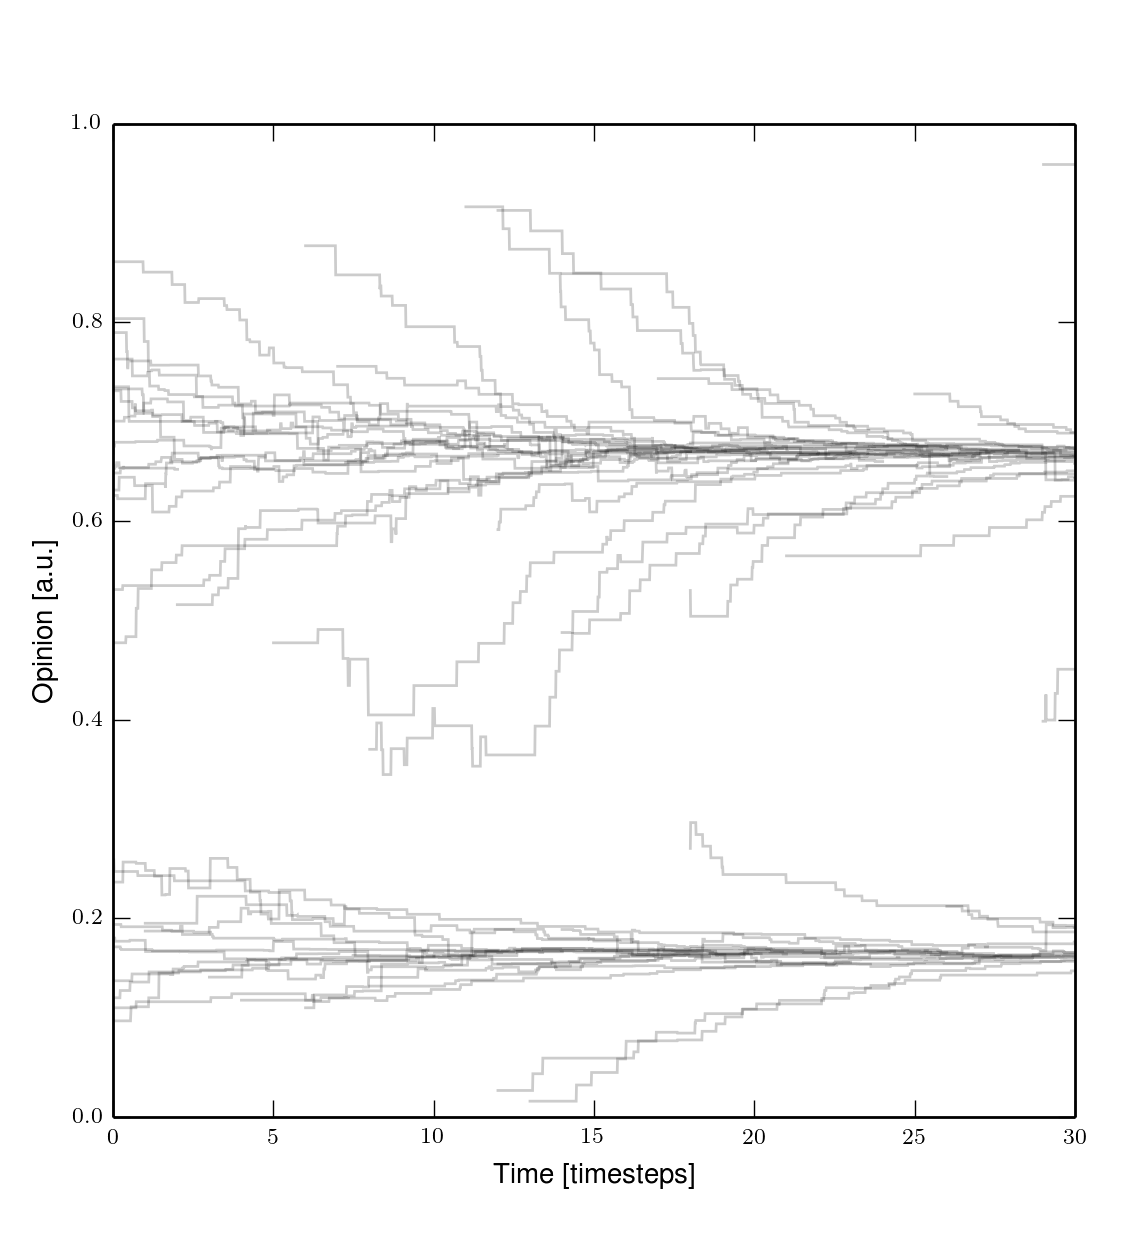
\includegraphics[height=0.9\textheight]{src/evol_03}
    \end{center}
    
%    \talk{ This is the evolution for $\varepsilon=0.5$.}

\end{frame}


\section{Grouping}
\begin{frame}\frametitle{Grouping With Hierarchical Clustering}
    % left: equations
    \begin{columns}[c,onlytextwidth]
        \begin{column}[t]{5cm}
            A group features
            \begin{itemize}
                \item at least 2 agents
                \item no bigger distance between members than to the
                nearest non-member
            \end{itemize}
        \end{column}
        \begin{column}[t]{5cm}
            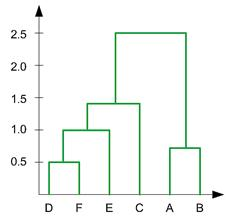
\includegraphics[width=0.9\textwidth]{src/cluster.jpg}
        \end{column}
    \end{columns}
%   \talk{ What are these groups?}

\end{frame}

\begin{frame}\frametitle{Grouping in Action}
    \begin{center}
        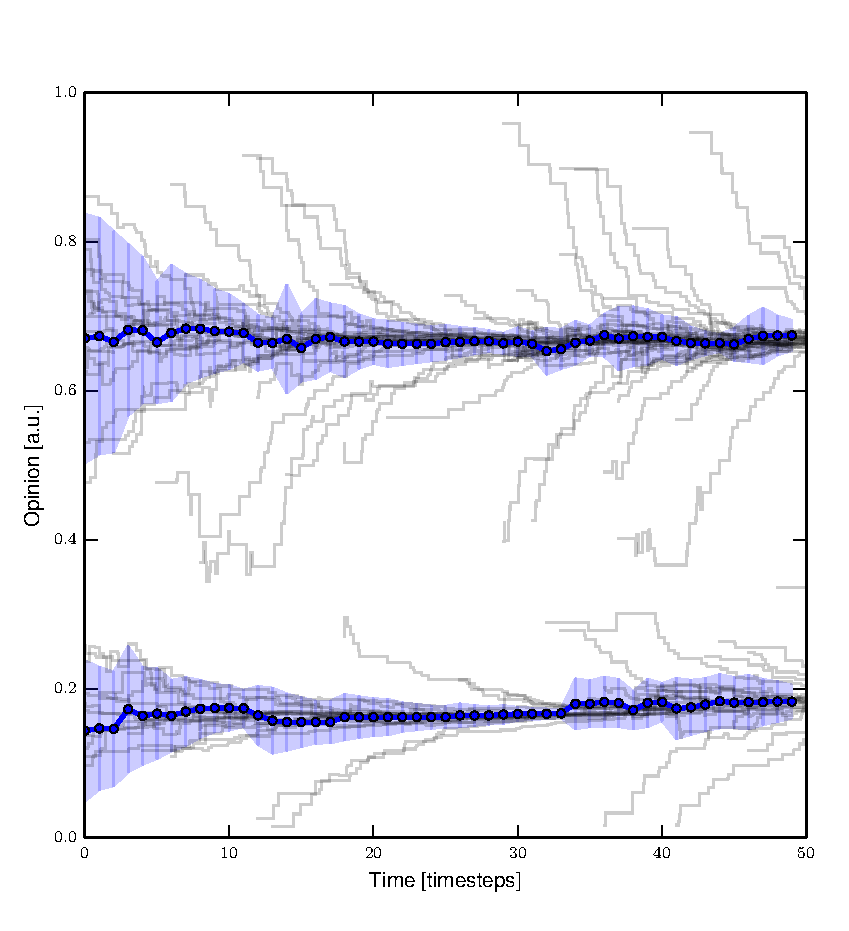
\includegraphics[height=0.8\textheight]{src/evol_03_groups.pdf}
    \end{center}
    
%    \talk{ These are the groups identified for $\varepsilon=0.5$.}

\end{frame}


\section{Group Evolution}
\begin{frame}\frametitle{Group Evolution}
    % left: equations

    % right: picture
    \begin{center}
        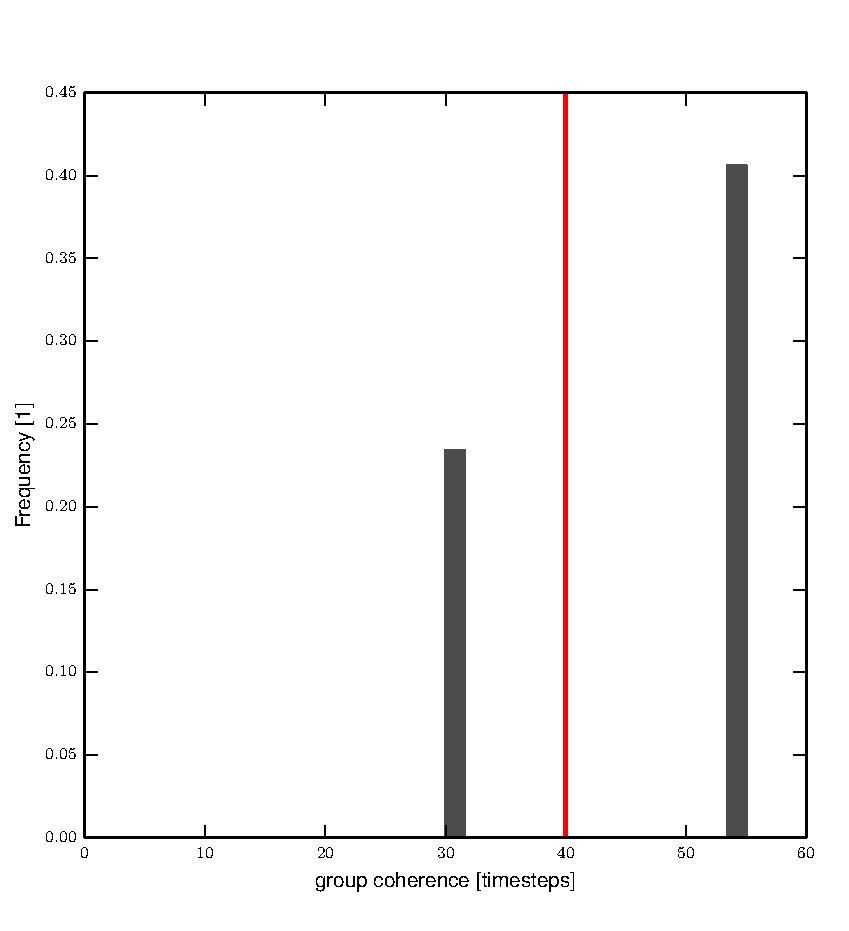
\includegraphics[height=0.8\textheight]{src/var_03.pdf}
    \end{center}
    
%    \talk{Timescale before significant change happens}

\end{frame}


\section{Analytic Treatment}
\begin{frame}\frametitle{Analytic Treatment: Steady State}
    % steady state: Brownian motion
    \vskip1em
    \begin{itemize}
        \item Brownian Motion
        \begin{equation*}
            E(|O_i(T+\Delta T)-O_i(T)|) = \sqrt{\frac{2\Delta T}{\pi}\frac{\varepsilon \zeta}{2 N_i}}
        \end{equation*}
        \item mean step size is $\varepsilon \zeta /(2 N_i)$
        \item merging with adjacent group after diffusion over $\varepsilon/2$
        \item change timescale from diffusion and merging time-scales
        \begin{eqnarray*}
            \Delta T &\approx& \frac{\pi}{4}\frac{N_i\varepsilon}{\zeta} + T_p\\
            T_p&=&\frac{N_i(T)}{N_{\rm tot}}\cdot N_{\rm it. per timestep}\cdot \zeta
        \end{eqnarray*}
        \item fiducial configuration $\varepsilon=0.25$, $\zeta=0.1$, $N_i\approx 50\cdot
2\varepsilon = 25$
        \begin{equation*}
            \Delta T=40+5=45
        \end{equation*}
     \end{itemize}

%    \talk{What do we expect?}

\end{frame}


\section{Fiducial Simulation}
\begin{frame}\frametitle{Fiducial Simulation}
    \begin{center}
        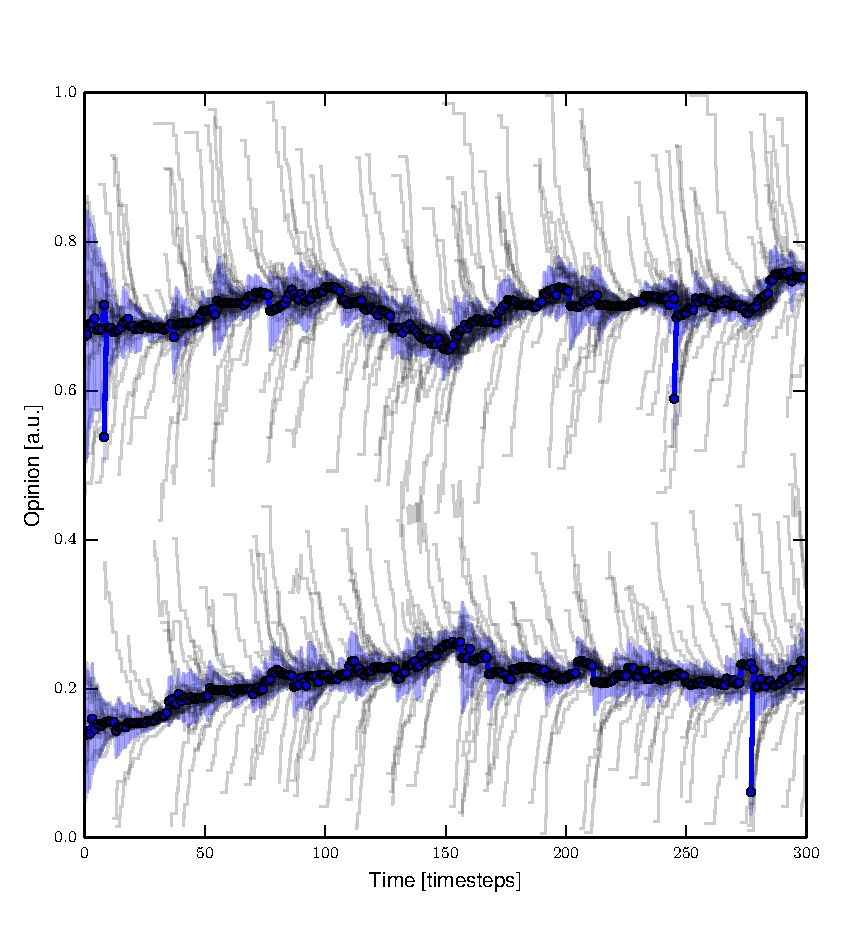
\includegraphics[width=0.5\textwidth]{src/fiducial.pdf}
        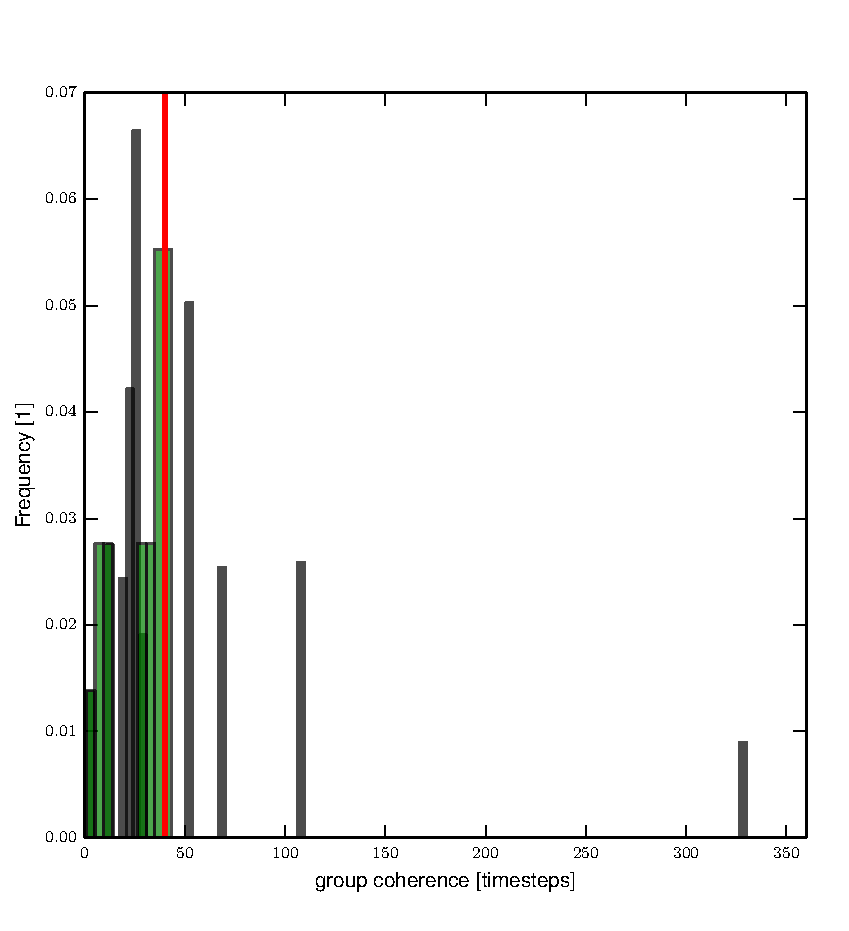
\includegraphics[width=0.5\textwidth]{src/fiducial_var_th.pdf}
    \end{center}
    \begin{itemize}
        \item $a_{\rm max}=40$, $\varepsilon=0.25$, $\zeta=0.1$,
        $N_{\rm tot}=50$, $T_{\rm max}=300$
    \end{itemize}
%    \talk{}

\end{frame}

\section{Parameter Sweep}
\begin{frame}\frametitle{Low $a_{\rm max}=20$}
    \begin{center}
        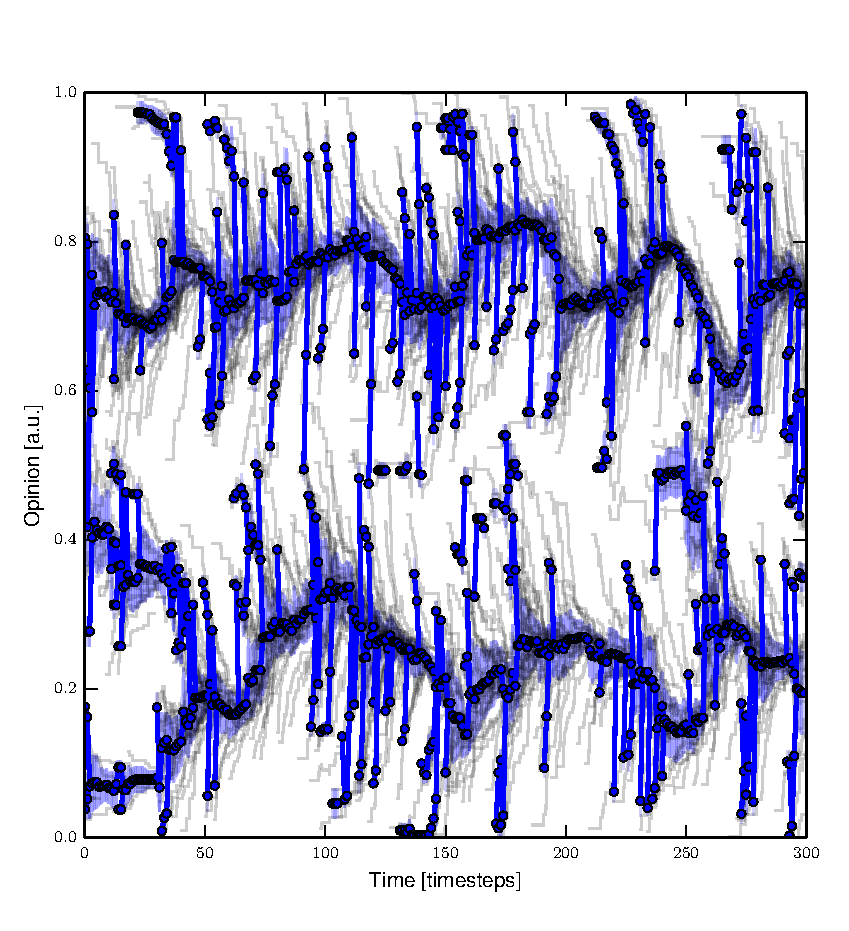
\includegraphics[width=0.5\textwidth]{fig/evol_20.pdf}
        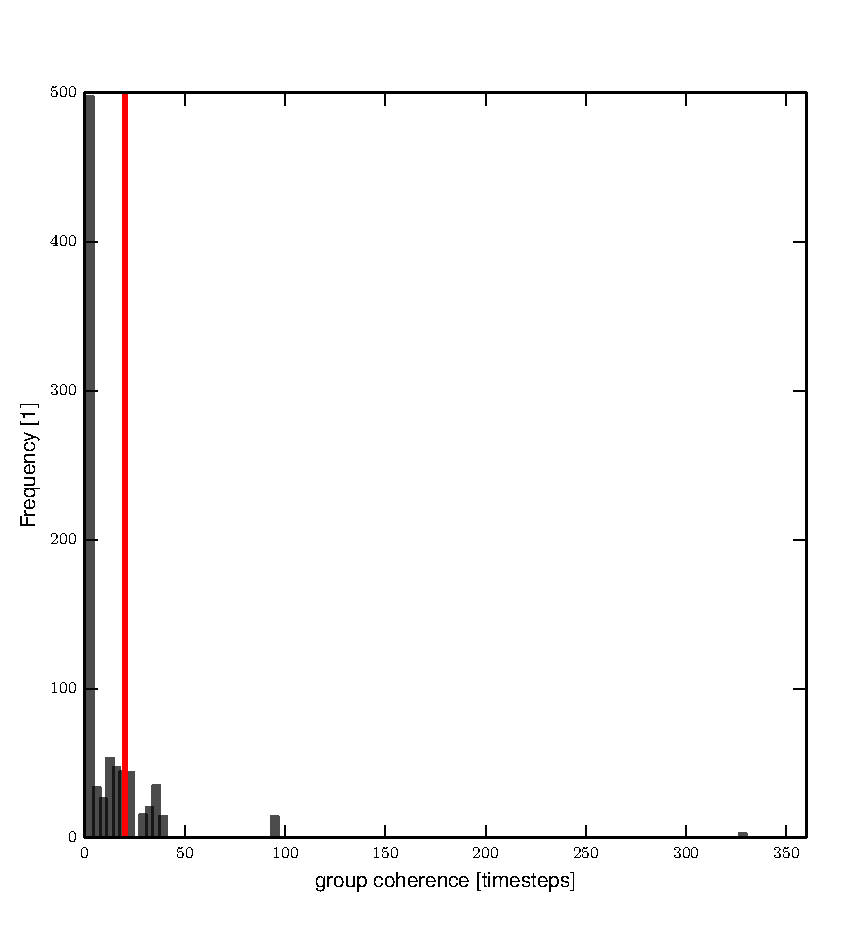
\includegraphics[width=0.5\textwidth]{fig/var_20.pdf}
    \end{center}

%    \talk{}

\end{frame}

\begin{frame}\frametitle{High $a_{\rm max}=80$}
    \begin{center}
        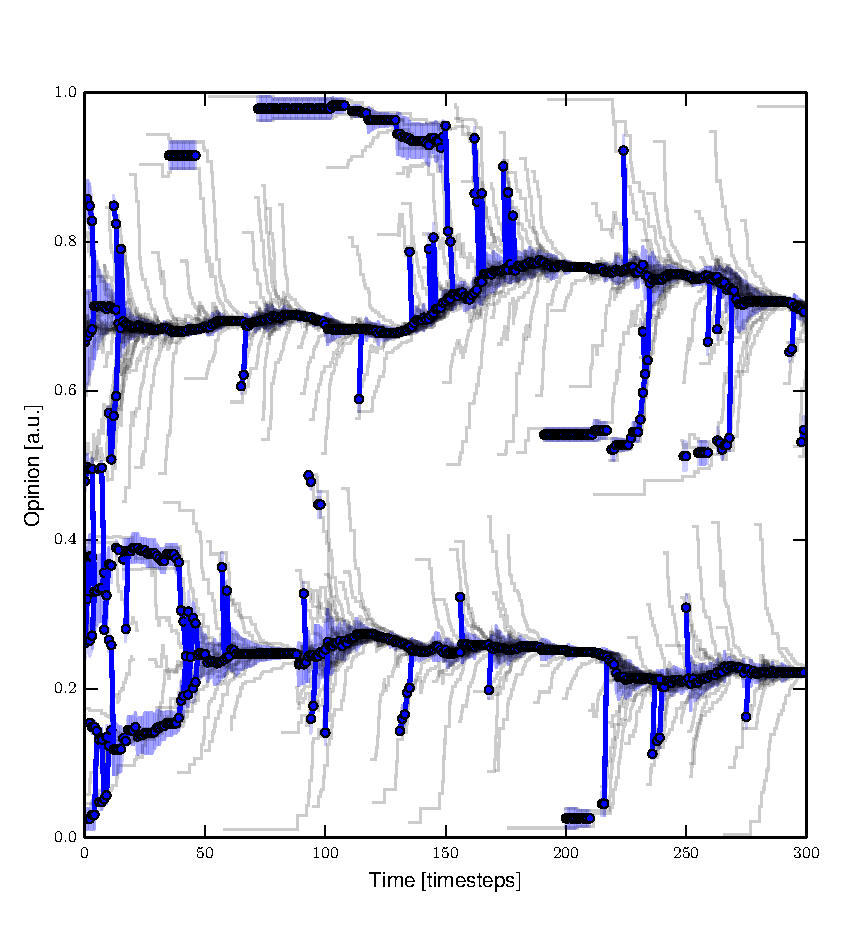
\includegraphics[width=0.5\textwidth]{fig/evol_80.pdf}
        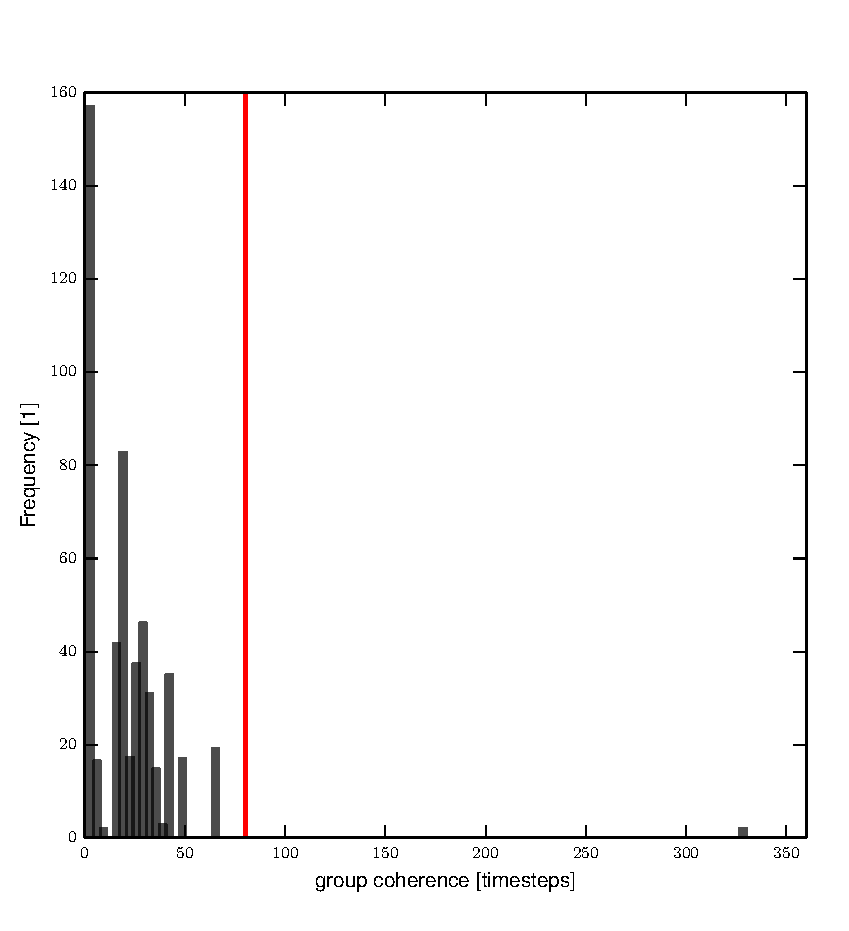
\includegraphics[width=0.5\textwidth]{fig/var_80.pdf}
    \end{center}

%    \talk{}

\end{frame}

\begin{frame}\frametitle{Low $\varepsilon=0.1$}
    \begin{center}
        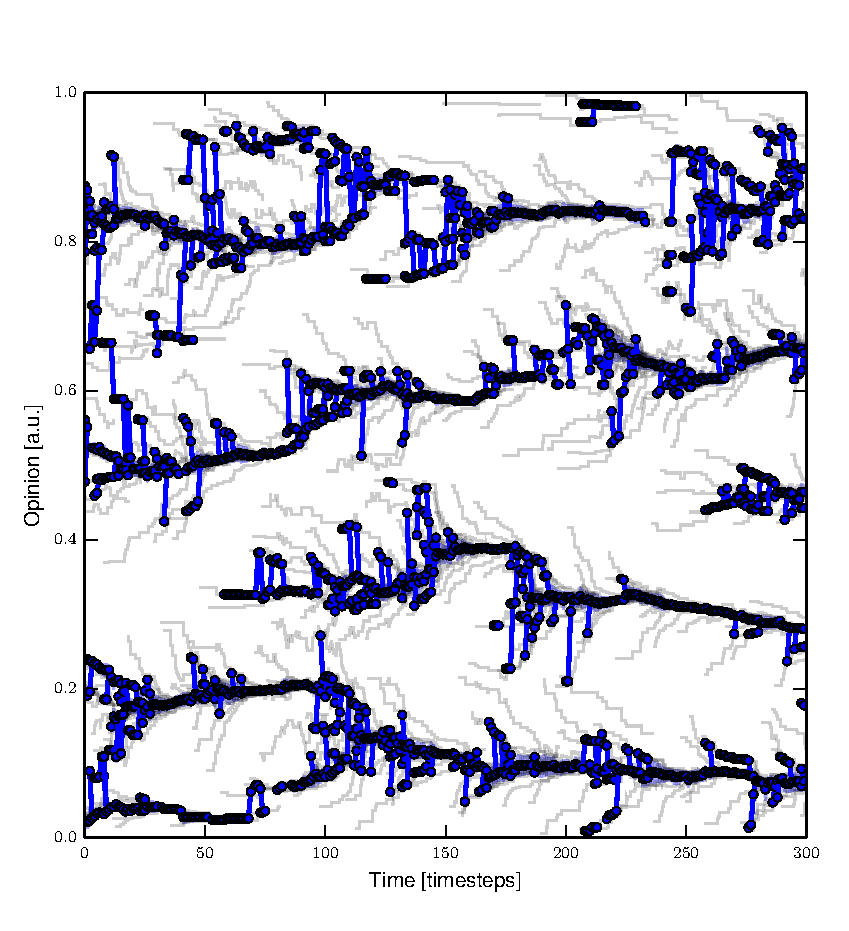
\includegraphics[width=0.5\textwidth]{fig/evol_01.pdf}
        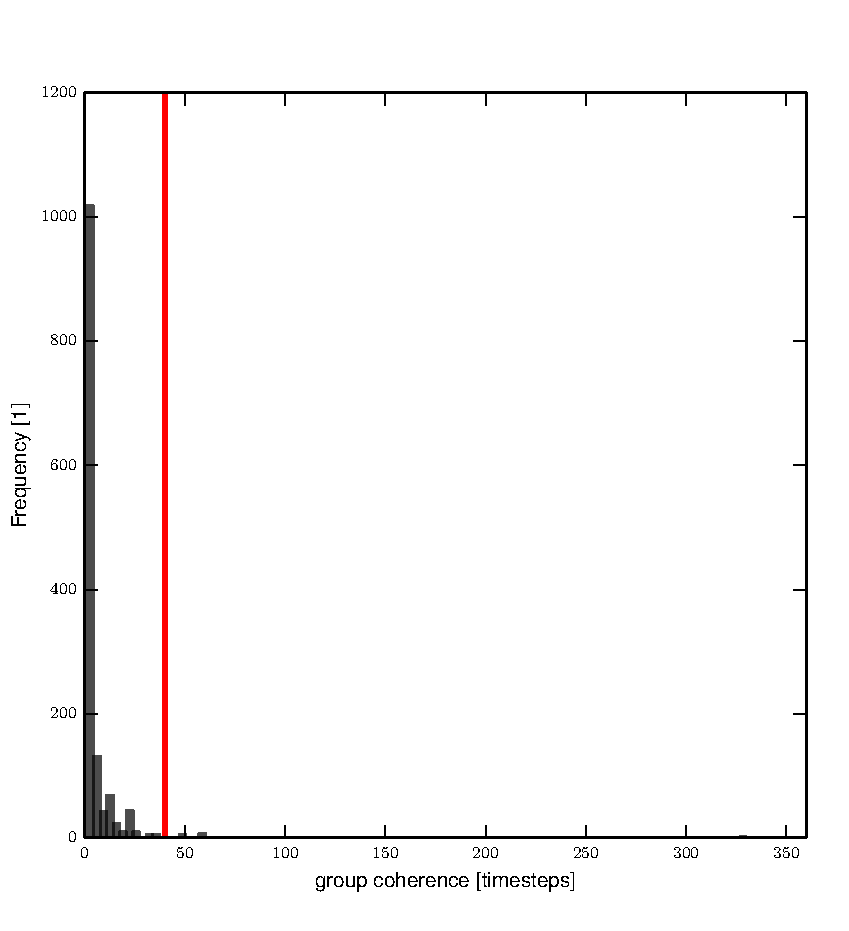
\includegraphics[width=0.5\textwidth]{fig/var_01.pdf}
    \end{center}

%    \talk{}

\end{frame}

\begin{frame}\frametitle{High $\varepsilon=0.4$}
    \begin{center}
        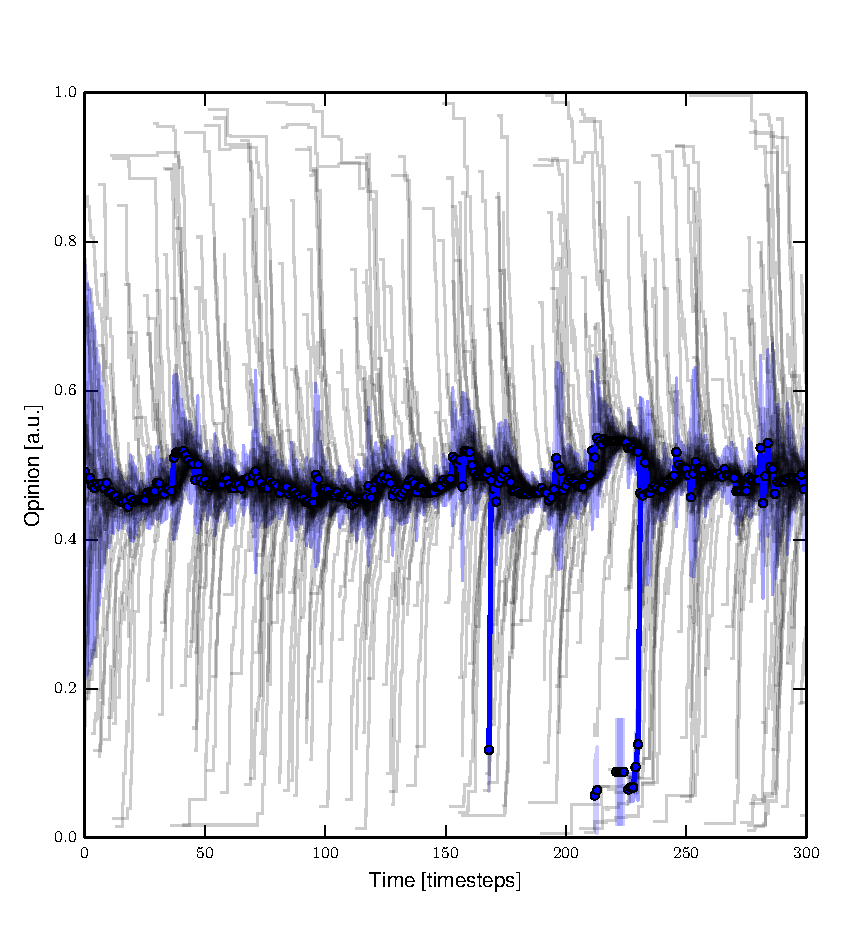
\includegraphics[width=0.5\textwidth]{fig/evol_04.pdf}
        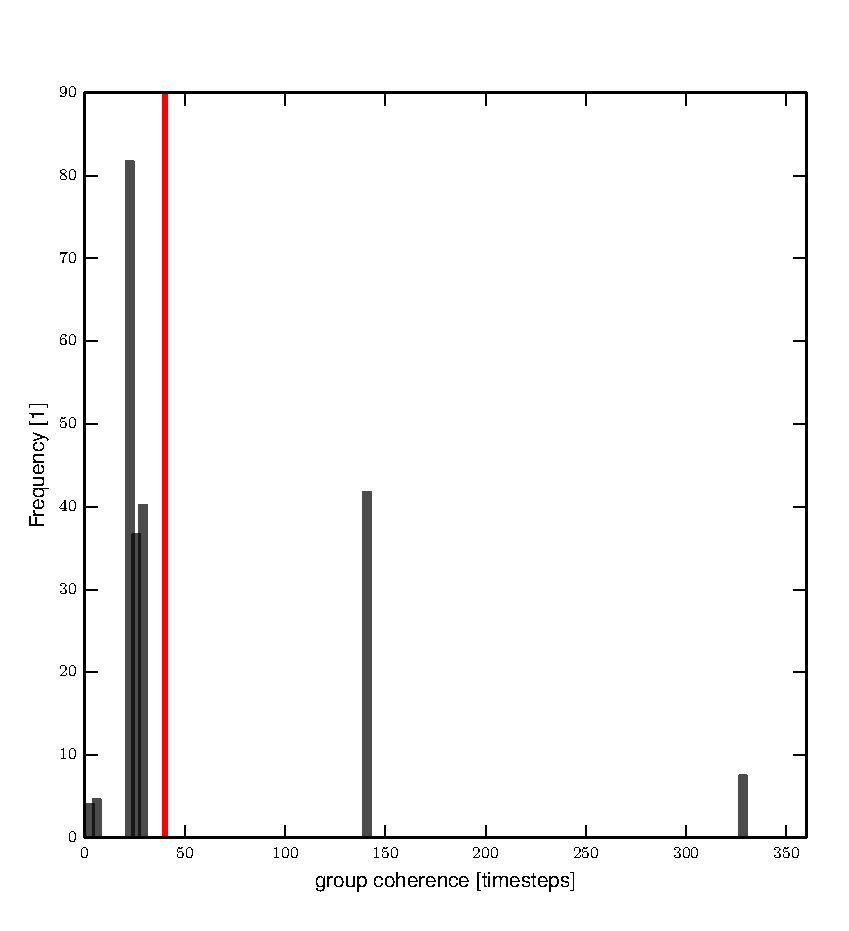
\includegraphics[width=0.5\textwidth]{fig/var_04.pdf}
    \end{center}

%    \talk{}

\end{frame}

\section{Discussion}
\begin{frame}\frametitle{Summary}
    \begin{itemize}
        \item evolution of group opinion happens
        \item on timescales $\Delta T\in [0, 3 a_{\rm max}]$
        \item important parameters: $\varepsilon$, noise $1/a_{\rm max}$
    \end{itemize}
    \begin{center}
        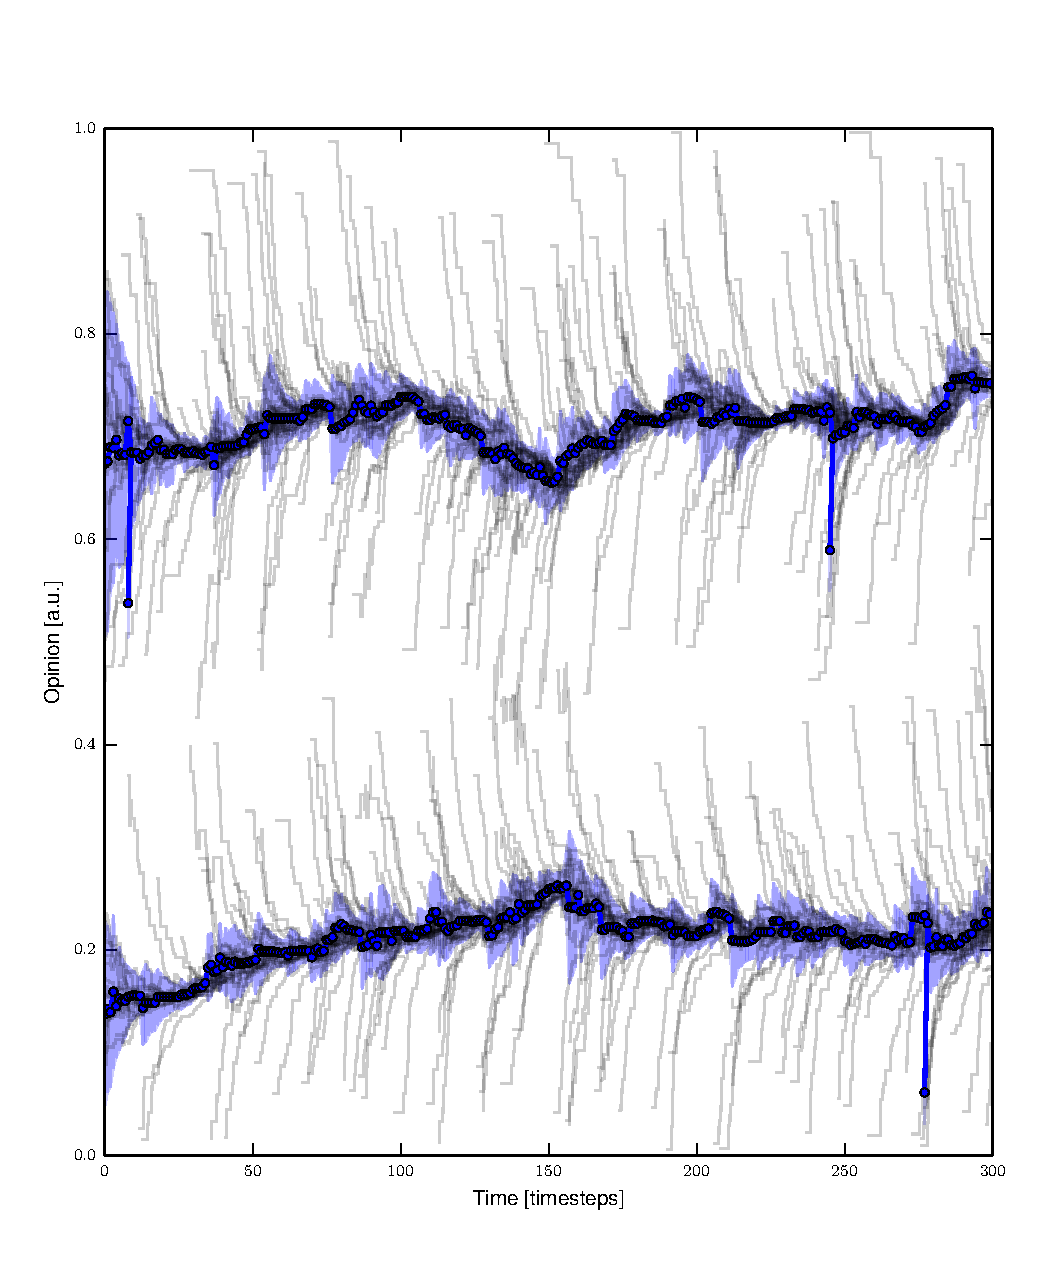
\includegraphics[width=0.4\textwidth]{fig/fiducial.pdf}
        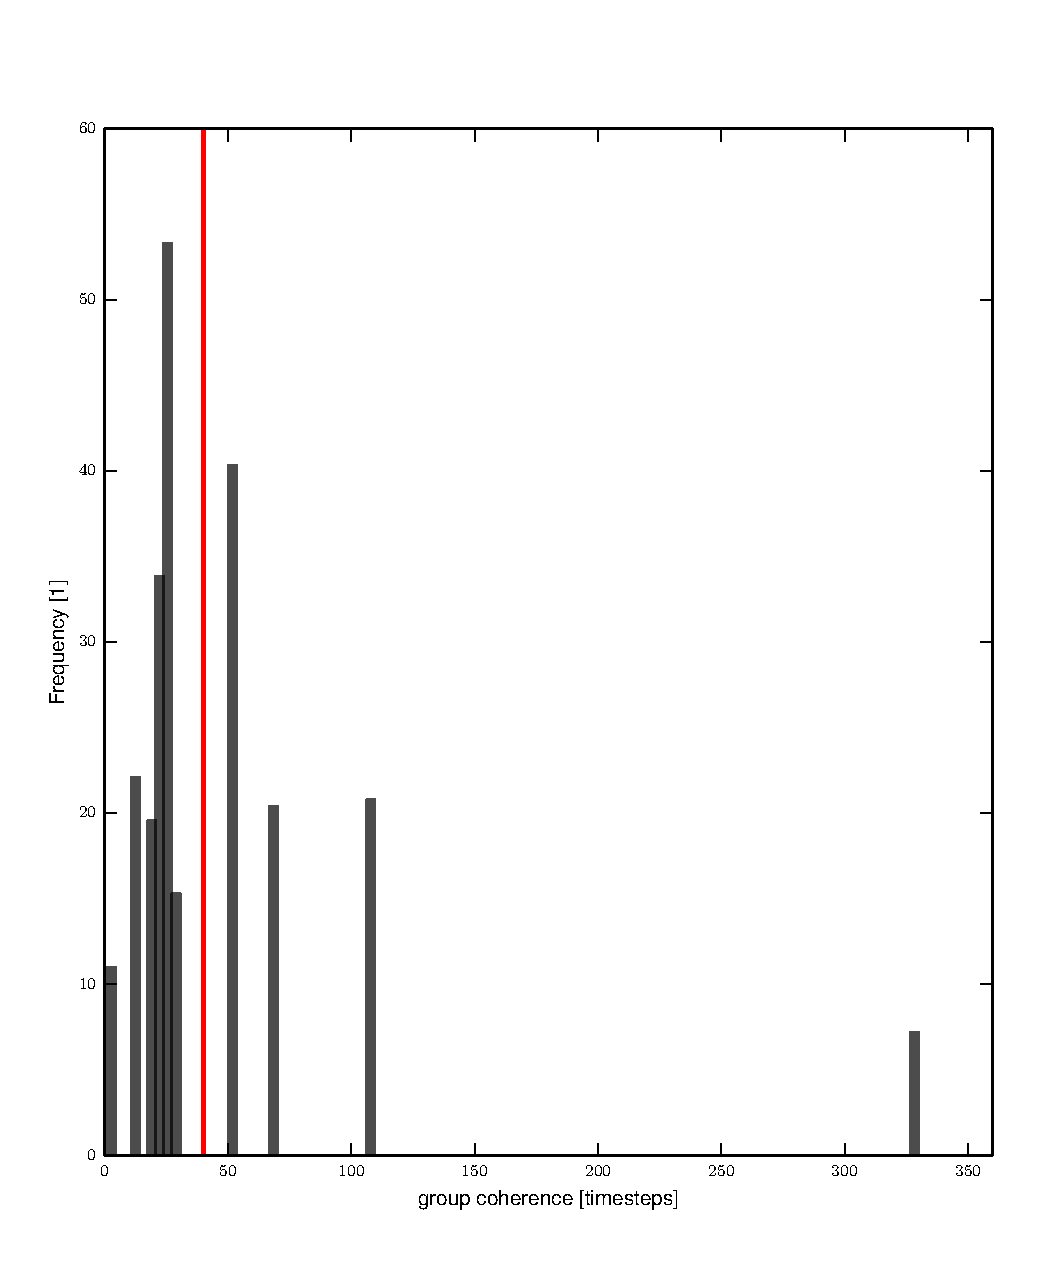
\includegraphics[width=0.4\textwidth]{fig/fiducial_var.pdf}
    \end{center}

%    \talk{}

\end{frame}


\end{document}
